\section{Manual}
\numberwithin{figure}{subsubsection}
\subsection{Deployment}

\emph{localhost} is deployed using Amazon Web Services on an Amazon Elastic
Compute Cloud instance with the following specifications.
\begin{lstlisting}
OS: Ubuntu 18.04.1 LTS x86_64
Host: HVM domU 4.2.amazon
Kernel: 4.15.0-1023-aws
CPU: Intel Xeon E5-2676 v3 (1) @ 2.4
GPU: Cirrus Logic GD 5446
Memory: 983MiB
\end{lstlisting}

\subsubsection{Amazon Web Services Configuration}

After creating an Amazon Elastic Compute Cloud instance through the Amazon Web
Services dashboard, the only port on the server accessible from the internet
is \lstinline{22 (SSH)}. For the server to accept web requests, ports
\lstinline{80 (HTTP)} and \lstinline{443 (SSL)} must be opened. This can be
done by navigating to the dashboard, selecting the running
\emph{Amazon Elastic Compute Cloud} instance, and selecting
\lstinline{launch-wizard}. A tab will then appear at the bottom of the page
and will contain a form that can open ports.

\subsubsection{Software}

While a number of scripts are provided to automate the installation and
configuration of \emph{localhost}, some manual configuration is required.
The configuration required varies between different Linux distribution so the
following steps are only supported on Ubuntu 18.04.1.

The default user account provided on an Amazon Elastic Compute Cloud instance
running Ubuntu 18.04.1 is \lstinline{ubuntu} and the following commands rely on
this assumption. Commands requiring sudo privileges are prepended with
\lstinline{#} and commands executed under user permissions are prepended with
\lstinline{$}.

\paragraph{Update}

The initial state of the instance is likely out of date and should be brought
up to date by running the following command.
\begin{lstlisting}
# apt update && apt upgrade && apt dist-upgrade && apt autoremove
\end{lstlisting}

\paragraph{Repository}

To ease updating, an SSH key will be generated to authenticate the server when
accessing the repository.
\begin{lstlisting}
$ ssh-keygen -t rsa -b 4096
Enter file in which to save the key (/home/ubuntu/.ssh/id_rsa):
Enter passphrase (empty for no passphrase):
Enter same passphrase again:
Your identification has been saved in id_rsa.
Your public key has been saved in id_rsa.pub.
\end{lstlisting}
After adding \lstinline{/home/ubuntu/.ssh/id_rsa.pub} to BitBucket the
repository can be cloned.
\begin{lstlisting}
$ git clone git@bitbucket.org:jtalowell/localhost.git /home/ubuntu/localhost
\end{lstlisting}

\paragraph{Django \& Immediate Dependencies}

To install a virtual environment and manage dependencies the following
packages must be installed.
\begin{lstlisting}
# apt install python3-venv python3-pip
\end{lstlisting}
Django and its immediate dependencies can then be installed.
\begin{lstlisting}
$ cd /home/ubuntu/localhost
$ python3 -m venv venv
$ source venv/bin/activate
$ (venv) pip install -r requirements.txt
\end{lstlisting}

\paragraph{PostgreSQL}

PostgreSQL must be installed and it's accompanying system service enabled.
\begin{lstlisting}
# apt install postgresql postgresql-contrib
# systemctl enable postgresql.service
# systemctl start postgresql.service
\end{lstlisting}
The database cluster can then be created.
\begin{lstlisting}
$ sudo -u postgres -i
[postgres]$ /usr/lib/postgresql/10/bin/initdb -D '/var/lib/postgresql/data'
\end{lstlisting}
A user to administer the database clusted must be created for access.
\begin{lstlisting}
[postgres]$ createuser --interactive
Enter name of role to add: ubuntu
Shall the new role be a superuser? (y/n) y
[postgres]$ exit
\end{lstlisting}
The database to use for the project can now be created.
\begin{lstlisting}
$ createdb localhost_db
$ sudo -u postgres -i
[postgres]$ psql
postgres=# \password ubuntu
Enter new password: [DB_PW]
Enter it again: [DB_PW]
postgres=# GRANT ALL PRIVILEGES ON DATABASE localhost_db TO ubuntu;
postgres=# ALTER ROLE ubuntu SET client_encoding TO ``utf8'';
postgres=# ALTER ROLE ubuntu SET default_transaction_isolation TO ``read committed'';
postgres=# \q
[postgres]$ exit
\end{lstlisting}

\paragraph{Redis}

Ubuntu's package for Redis works without any extended configuration and its
services are automatically started and enabled.
\begin{lstlisting}
# apt install redis-server
\end{lstlisting}

\paragraph{Daphne}

Daphne is installed as one of Django's immediate dependencies.
A service script is provided for installation.
\begin{lstlisting}
# ln -sf /home/ubuntu/localhost/deploy/systemd/daphne.service /etc/systemd/system/
# vim /etc/systemd/system/daphne.service
\end{lstlisting}
The environment variables for \lstinline{SECRET_KEY}, \lstinline{DB_USER}, and
\lstinline{DB_PW} must be set for Daphne to be able to operate. This
can be done by inserting the following lines in the service script.
\begin{lstlisting}
Environment="SECRET_KEY=YOUR KEY HERE"
Environment="DB_USER=ubuntu"
Environment="DB_PW=YOUR DB PASSWORD HERE"
\end{lstlisting}

\paragraph{Gunicorn}

Gunicorn, like Daphne, is installed as one of Django's immediate dependencies.
A service script is provided for installation.
\begin{lstlisting}
# ln -sf /home/ubuntu/localhost/deploy/systemd/gunicorn.service /etc/systemd/system/
# vim /etc/systemd/system/gunicorn.service
\end{lstlisting}
The environment variables for \lstinline{SECRET_KEY}, \lstinline{DB_USER},
and \lstinline{DB_PW} must be set for Gunicorn to be able to operate.
This can be done by inserting the following lines in the service script.
\begin{lstlisting}
Environment="SECRET_KEY=YOUR KEY HERE"
Environment="DB_USER=ubuntu"
Environment="DB_PW=YOUR DB PASSWORD HERE"
\end{lstlisting}

\paragraph{Celery}

Service scripts are provied for both Celery and Celery Beat.

\begin{lstlisting}
# ln -sf /home/ubuntu/localhost/deploy/systemd/celery.service /etc/systemd/system/
# ln -sf /home/ubuntu/localhost/deploy/systemd/celery-beat.service /etc/systemd/system/
# vim /etc/systemd/system/celery.service
# vim /etc/systemd/system/celery-beat.service
\end{lstlisting}
The following must be added to both service scripts.
\begin{lstlisting}
Environment="SECRET_KEY=YOUR KEY HERE"
Environment="DB_USER=ubuntu"
Environment="DB_PW=YOUR DB PASSWORD HERE"
\end{lstlisting}


\paragraph{NGINX}

NGINX can be installed using the following commands.
\begin{lstlisting}
# apt install nginx
# systemd enable nginx
# systemd start nginx
\end{lstlisting}

The relevant configuration files can be installed by:
\begin{lstlisting}
# /home/ubuntu/localhost/deploy/init.sh
\end{lstlisting}
\emph{localhost} uses Let's Encrypt as the provider for it's SSL certificates.
The certificates can be installed using the Certbot tool which can be
installed and executed by the following commands. For this to work, the domain
name registered for \emph{localhost} should direct to the IP address of the
Amazon Elastic Compute Cloud instance.
\begin{lstlisting}
# apt install software-properties-common
# add-apt-repository ppa:certbot/certbot
# apt update
# apt install python-certbot-nginx
# certbot --nginx certonly
\end{lstlisting}
After installing the certificate the \lstinline{init.sh} script should be
executed again.
\begin{lstlisting}
# /home/ubuntu/localhost/deploy/init.sh [SECRET_KEY] [DB_USER] [DB_PW]
\end{lstlisting}
This script first ensures that the NGINX configuration script is installed
and restarts all the services that \emph{localhost} depends on.

\paragraph{Maintenance}

There are two scripts that are provided to ease server upgrades and deployment
testing. The first script is \lstinline{rebuild.sh}. This script automates the
dropping, creation, migrations, and loading of test data for the database.
This is useful for quickly loading a usable set of test data without manually
creating listings and accounts. It's also extendable to restore backups.
\begin{lstlisting}
-M is short for --Makemigrations
-m is short for --migrate
-s is short for --server and should only be used on the server deployment
-l is short for --loaddata and loads both testdata and propertyimages
\end{lstlisting}

The second script has already been mentioned but remains relevent for future
updates. \lstinline{init.sh} should be ran every time any updates or upgrades
take place to restart the required services otherwise unexpected errors can
occur through caching. When making changes to scheduling times, the Celery
and Celery Beat services must be stopped prior to running the
\lstinline{init.sh} script.
\begin{lstlisting}
# /home/ubuntu/localhost/deploy/init.sh
\end{lstlisting}

\newpage
\subsection{User Manual}
\subsubsection{Registering for an Account}
Register for an account by clicking on the 'Register' link in the top right
corner of the page and providing your email address, full name and entering
your password. Upon success, you will be logged in and redirected to the
homepage.

\begin{figure}[!h]
  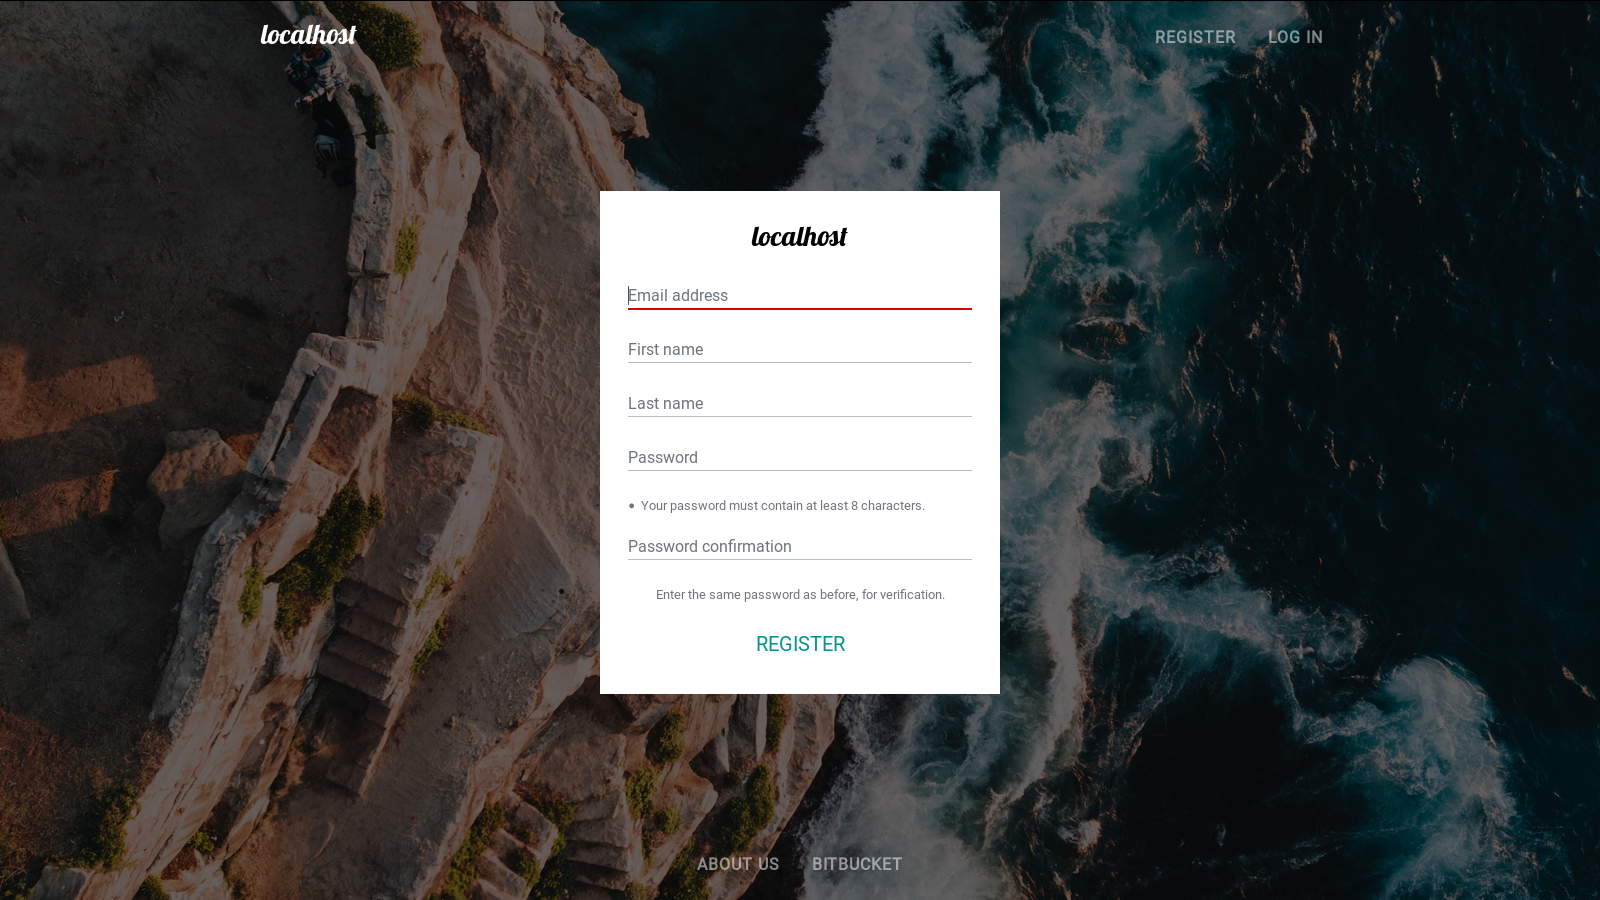
\includegraphics[width=\linewidth]{assets/userManual/regPg.png}
  \caption{Registration Page}
  \label{fig:regPg}
\end{figure}

\newpage
\subsubsection{Searching for a Property Item}
From the homepage, you can enter the location where you want to search around
and then either select it using the arrow keys and press enter, or click on the
search result and it will take you to the results page.

\begin{figure}[!h]
  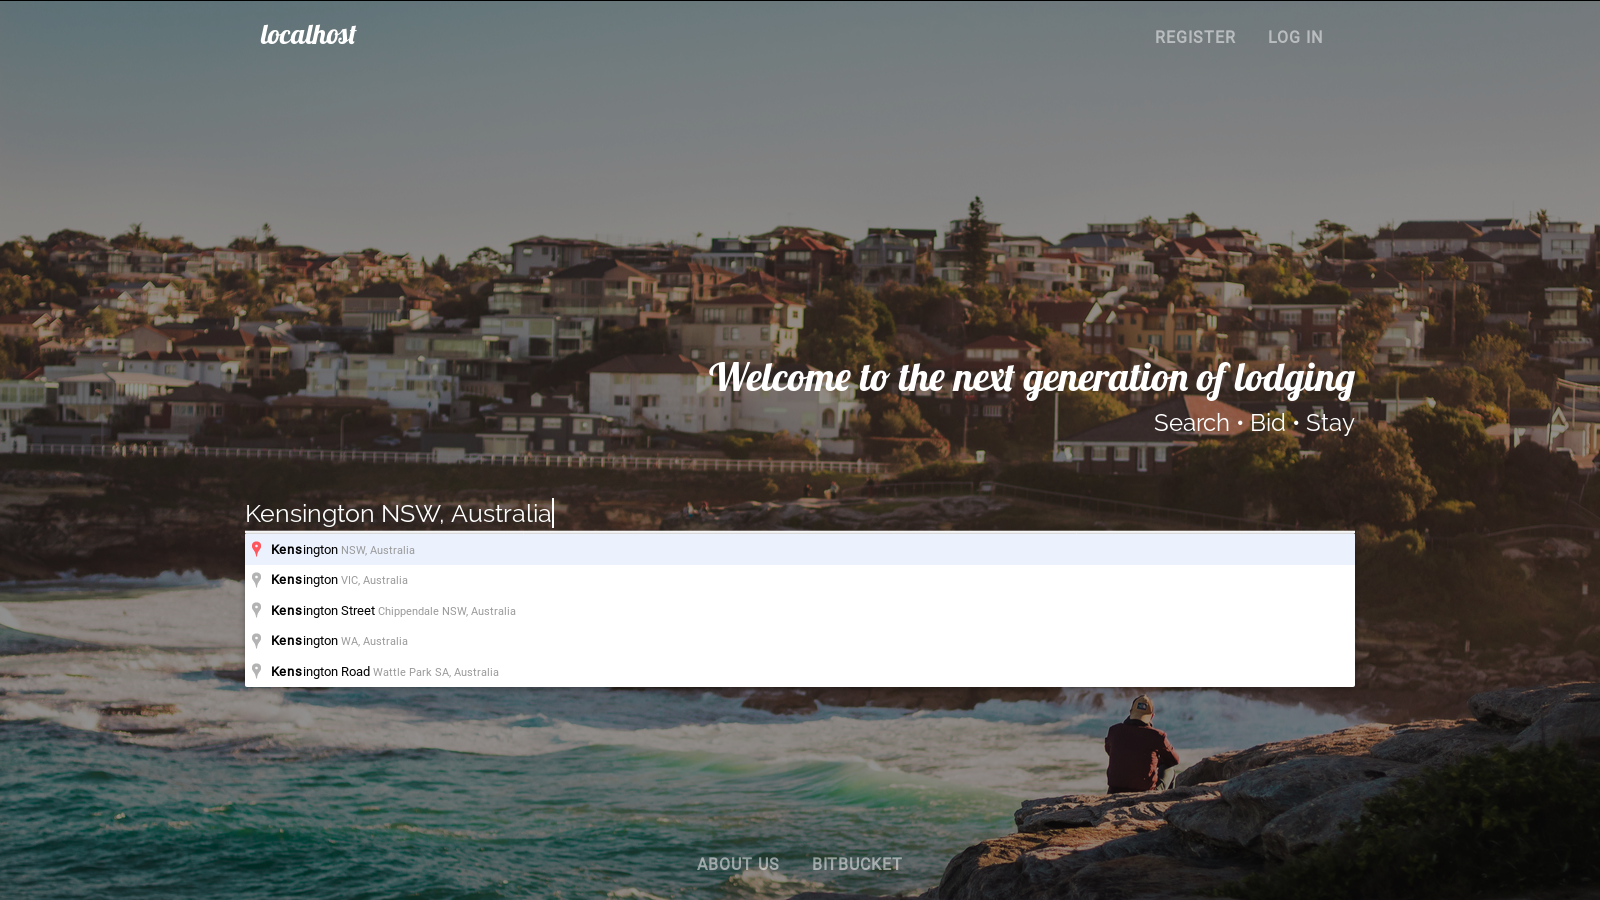
\includegraphics[width=\linewidth]{assets/userManual/searchOption.png}
  \caption{Selecting one of the search options}
  \label{fig:searchOption}
\end{figure}

Once you have reached the results page, all the properties will be ordered by
distance from the search location. From here, you can click on and apply
filters to the results such as specifying
the number of guests and/or toggling the results so that only properties with a
property item which is currently in an active bidding session will be displayed.

\begin{figure}[!h]
  
\includegraphics[width=\linewidth]{assets/userManual/searchFilters.png}
  \caption{Search filters}
  \label{fig:searchFilters}
\end{figure}

Upon choosing a property to view, you will be greeted by a carousel of images of
the property itself, information about the property including a map of it's
location, a picture of the host and methods to contact them, and the listings
currently available in that property.

\begin{figure}[!h]
  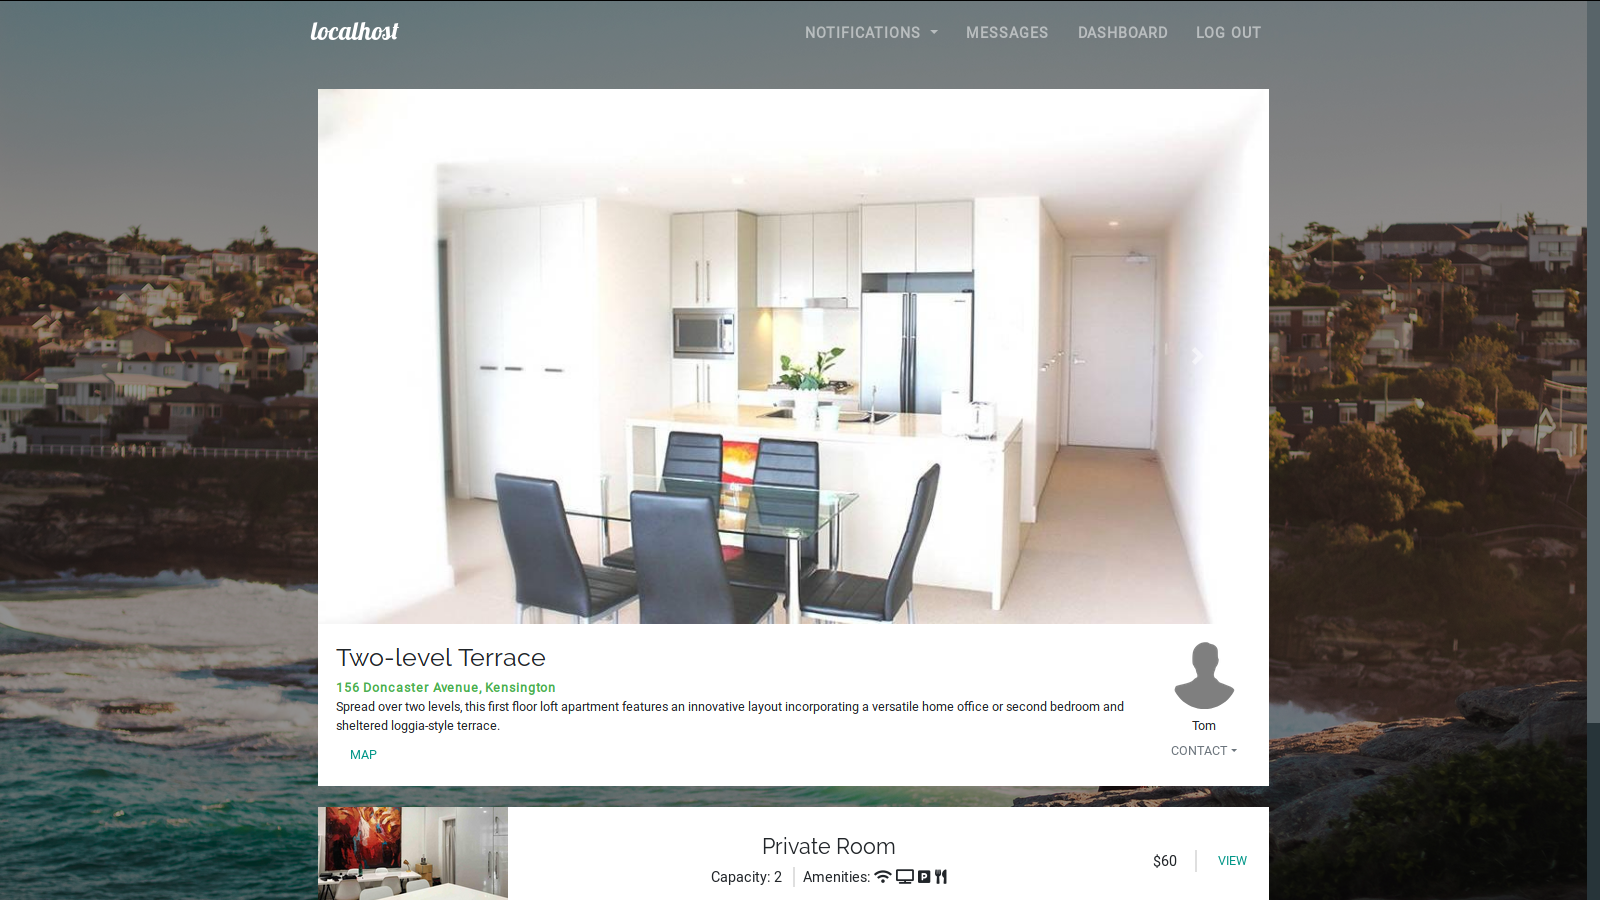
\includegraphics[width=\linewidth]{assets/userManual/propertyPg.png}
  \caption{Property images and details}
  \label{fig:propertyPg}
\end{figure}

To view a property item, click on the 'View' button to the far right of the row
of the row of the property item and a modal of the property will pop up.

\newpage
\subsubsection{Bidding on a Property Item}
To bid on a property item, you must be logged in, and viewing the relevant
property item's modal popup. Type a value which is greater than the current
highest bid and click on 'Place'. If someone bids higher than you, a
a notification will be sent to you.

\begin{figure}[!h]
  \centering
  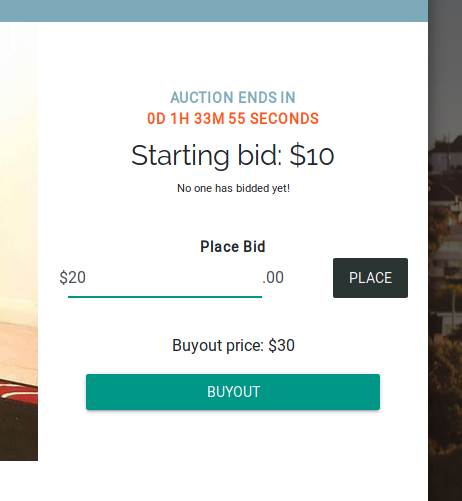
\includegraphics[height=8cm]{assets/userManual/biddingModule.png}
  \caption{Placing a bid on a property item}
  \label{fig:biddingModule}
\end{figure}

If there are any errors, there will be an alert pop up at the top of the
bidding module. Upon the end of a bidding session, all participants will receive
a notification indicating whether they have won or lost the auction.

\newpage
\subsubsection{Using the 'Buyout' Feature}
If you choose to buyout an auction, clicking on the 'Buyout' button will open
a confirmation dialog.

\begin{figure}[!h]
  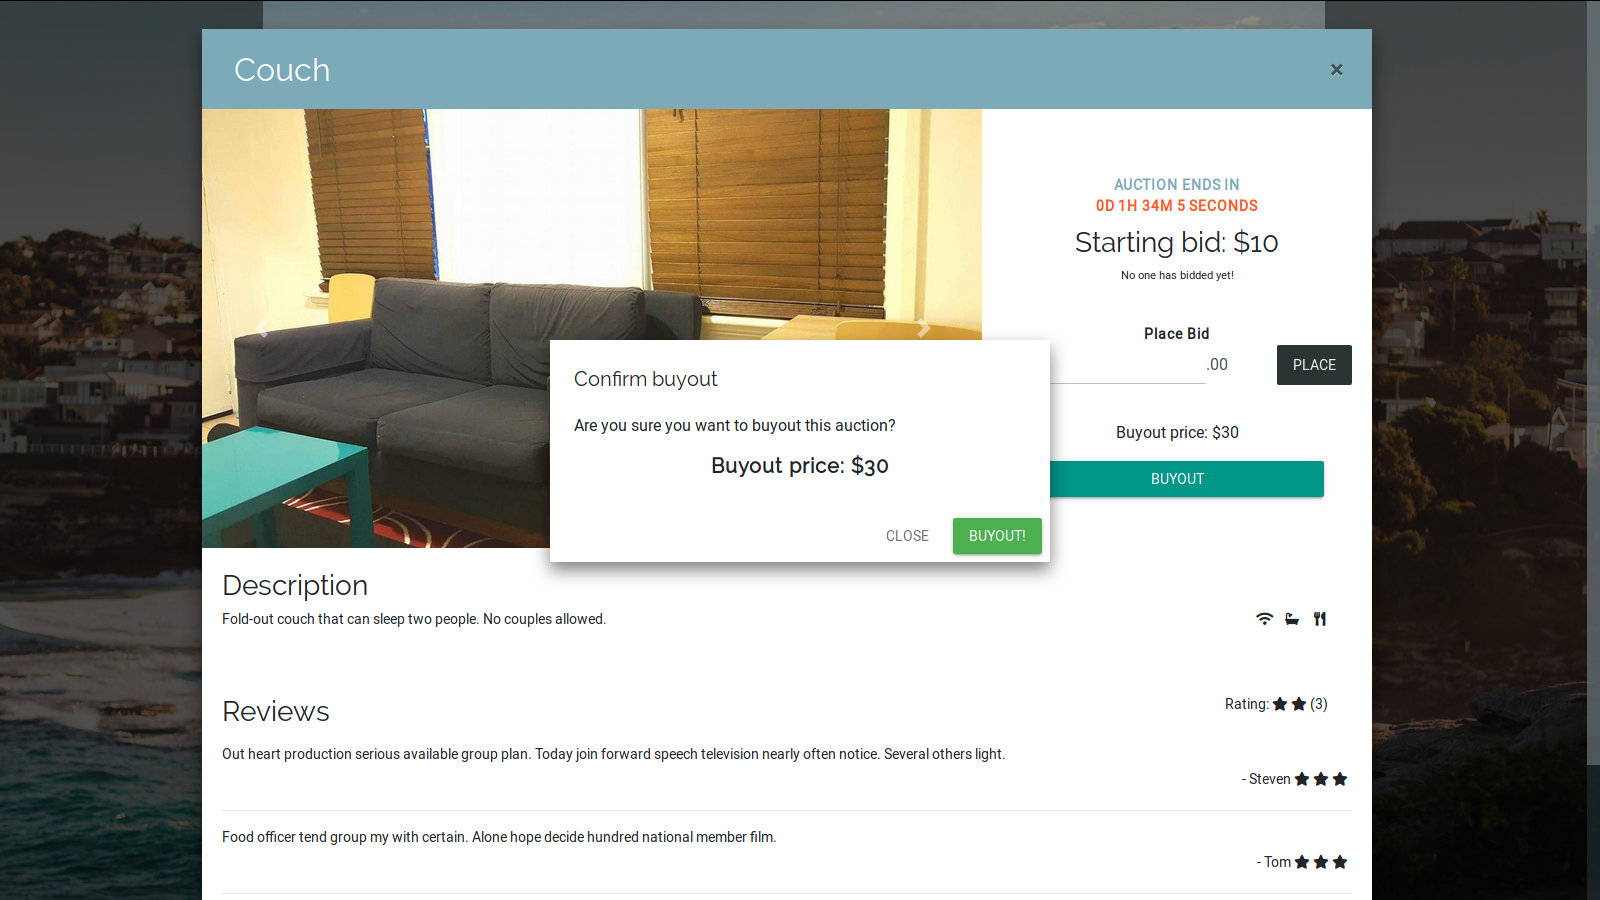
\includegraphics[width=\linewidth]{assets/userManual/buyoutConfirm.png}
  \caption{Confirmation pop up}
  \label{fig:buyoutConfirm}
\end{figure}

If the the buyout is confirmed, a notification will be
sent to all users who have placed a bid on this property item and the auction
will immediately close.

\newpage
\subsubsection{Contacting the Host}
From the property page, you can view the host's public profile by clicking on
the 'Contact' dropdown and selecting 'View host profile', or directly get in
touch by selecting 'Send a message'.

\begin{figure}[!h]
  \centering
  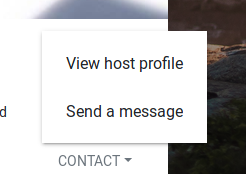
\includegraphics[height=7cm]{assets/userManual/contactHost.png}
  \caption{Options to contact a host}
  \label{fig:contactHost}
\end{figure}

Choosing the message the host will redirect you to the messaging page and a new
conversation with the host will be created. New incoming messages will move the
chat to the top of the contact list on the left of the messaging window. All
messages are in realtime so no refreshing of the page is required.

\newpage
\subsubsection{Using the Dashboard}
\paragraph{Active Bids}
This tab on the dashboard displays all of the properties that you have currently
placed a bid on. The price updates in real time, and you can navigate back to
the property by clicking on the property name.
\begin{figure}[!h]
  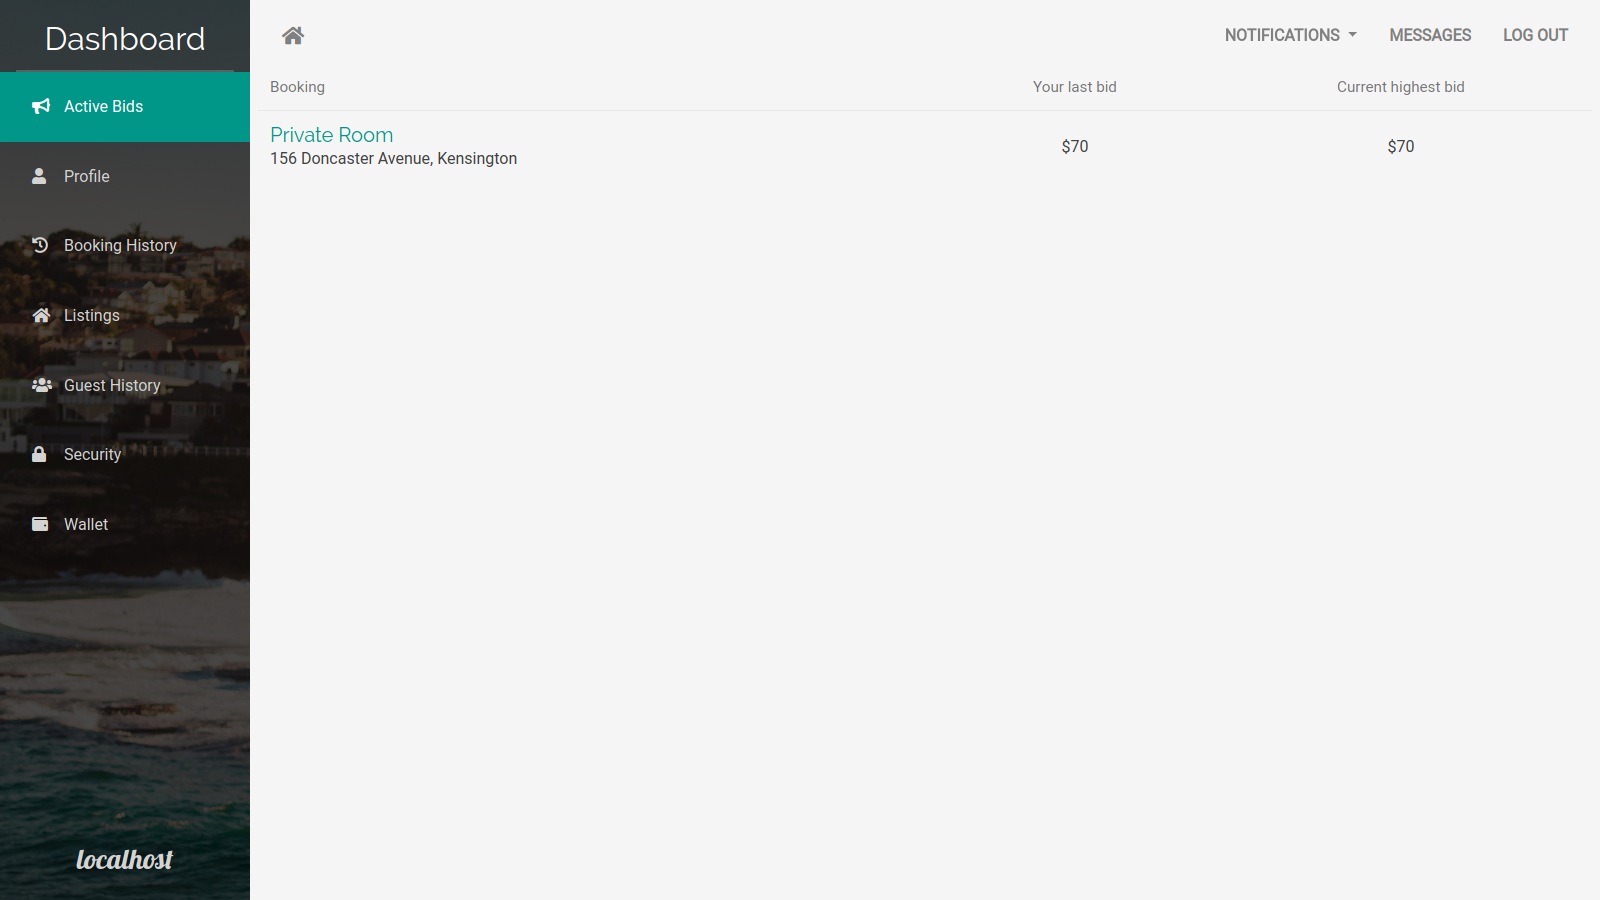
\includegraphics[width=\linewidth]{assets/userManual/activeBids.png}
  \caption{Active bids panel}
  \label{fig:activeBids}
\end{figure}

\paragraph{User Profile}
Update your personal description, date of birth and gender on this tab. Your
date of birth remains private, but your age will be displayed on your Public
Profile.

\paragraph{Booking History}
The booking history tab displays all of the previous places that you have stayed
at before. If the property is still being hosted, you can visit the property by
clicking on the name.
You can leave a review on the property once it is 24 hours past the checkin time.

\paragraph{Listings}
On the listings tab you can view all of the properties that you are hosting.

\paragraph{Guest History}
You can view the guests who have previously stayed at your properties. Clicking
on the user name will take you to their public profile.

\paragraph{Security}
Change your password in the Security tab by confirming your old and new passwords.

\paragraph{Wallet}
If you running low on funds, you can add more money to your wallet by entering
an amount on this tab.

\subsubsection{Adding a New Property}
To add a new property, visit the 'Listings' tab on the dashboard click on the
'Add Property' button in the bottom right corner of the screen. This will
redirect you to a new form to enter the property details and each property item
inside the property.

\begin{figure}[!h]
  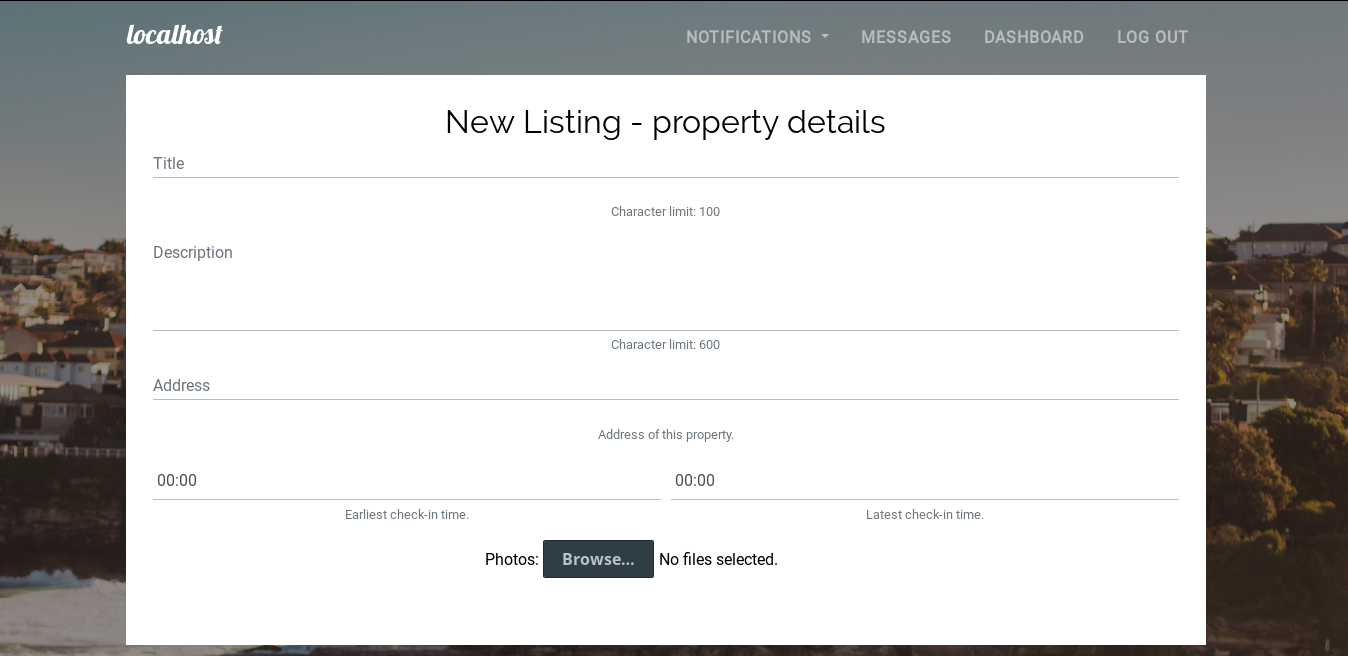
\includegraphics[width=\linewidth]{assets/userManual/newProperty.png}
  \caption{Adding a new property}
  \label{fig:newProperty}
\end{figure}

As seen below in the below figure, the '+Add Item' button adds another property
item to the property, while the 'Create Property' button will finalise everything
and create the listing.

\begin{figure}[!h]
  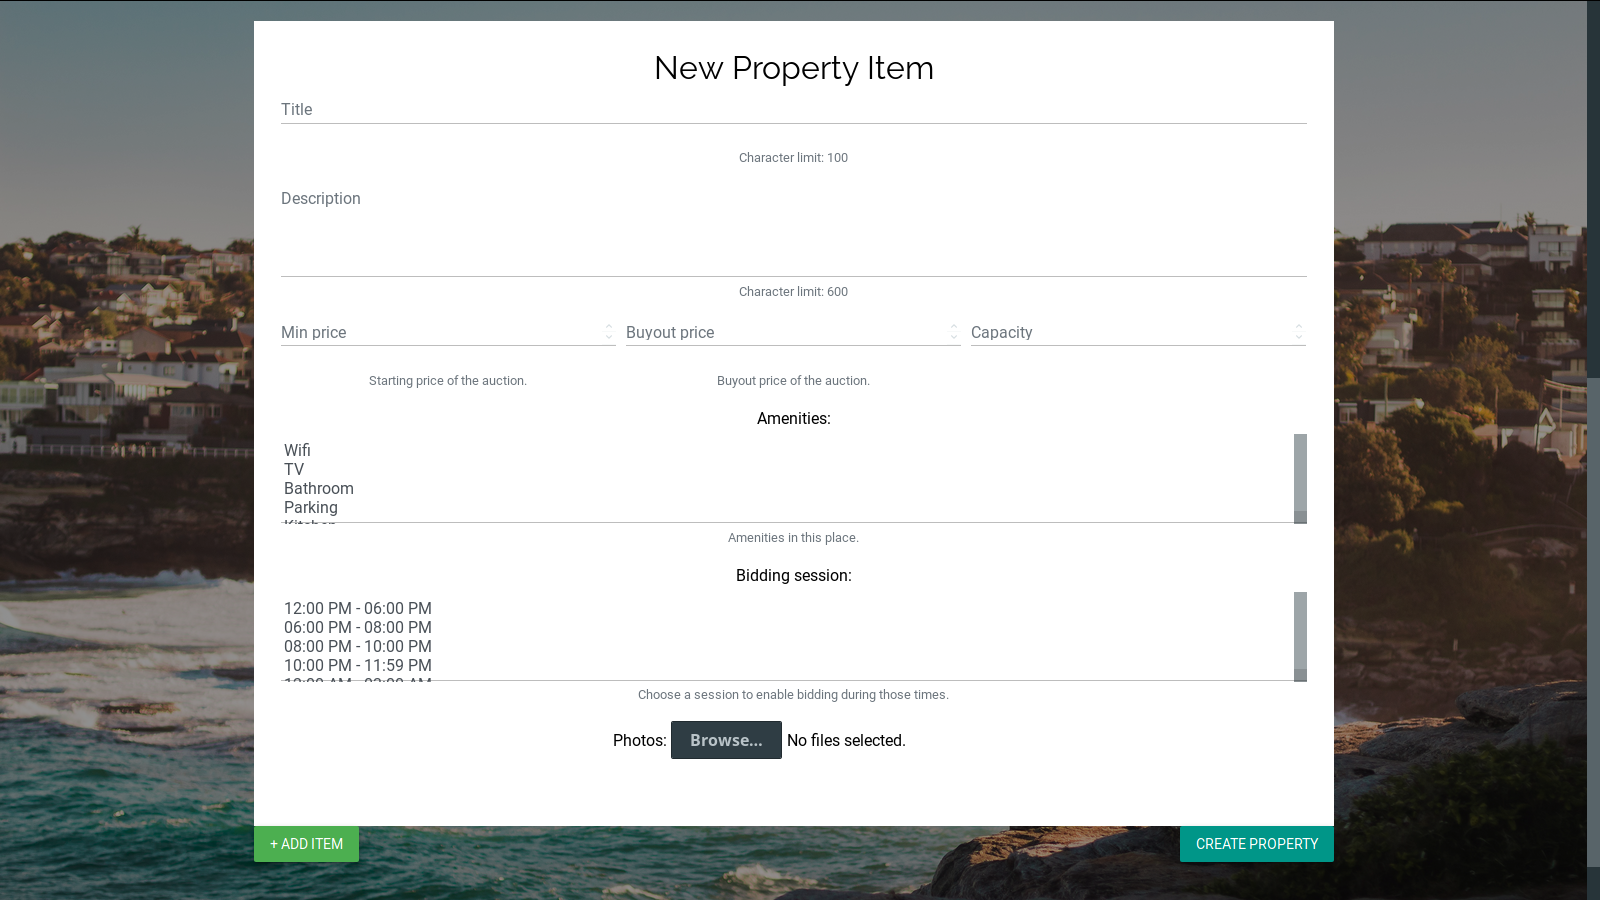
\includegraphics[width=\linewidth]{assets/userManual/newPropertyItem.png}
  \caption{Adding a new property item}
  \label{fig:newPropertyItem}
\end{figure}
